% \documentclass[a4paper]{article}
\documentclass[9pt,a4paper]{extarticle}

\usepackage{amsmath}
\usepackage{bm}
\usepackage{emposter}
\usepackage{multicol}
\usepackage{hyperref}
\usepackage{booktabs}
\usepackage{siunitx}
\usepackage{physics}

% \title{%
% Predicting composite ultimate strength with support vector machines:\\ a comparison of classical and quantum kernels%
% }
\title{%
Substructures as classifiers: predicting composites failure with\\ classical and quantum kernel methods%
}
\author{%
G.\ Tosti Balducci$^1$, B.\ Chen$^1$,
M.\ M\"{o}ller$^3$, M.\ Gerritsma$^2$,
R. de Breuker$^1$%
}
\affiliation{%
$^1$ TU Delft, Aerospace Structures and Materials\\%
$^2$ TU Delft, Flow Physics and Technology\\%
$^3$ TU Delft, Applied Mathematics%
}

\university{
\includegraphics[height=1.2\logoheight]{tudelft_logos/TUDelft_logo_black.eps}}
\rightlogo{}
\progresstype{PhD} % MSc, PhD, or PostDoc
\progresssections{4} % number of progress sections (years)
\progressfraction{3.9/4} % fraction of the bar to be filled

% %%%%%%%%%%%%%%%%%%%%%%%%%%%%%%%%%%%%%%%%%%%%%%%%%%%%%%%%%%%%%%%%%%%%%%%%%%%%%
\begin{document}
\maketitle
\begin{multicols}{2}
% %%%%%%%%%%%%%%%%%%%%%%%%%%%%%%%%%%%%%%%%%%%%%%%%%%%%%%%%%%%%%%%%%%%%%%%%%%%%%

% =============================================================================
\section{Motivation}
% =============================================================================
Full-scale finite element analyses capturing different physics at different scales are computationally expensive, if not unviable. A typical technique used to obviate to this problem is substructure homogenisation. This consists in replacing sections of a larger model with smaller higher-fidelity models, while setting the right internal boundary conditions. In recent times, data-trained machine learning models have been used as substructures \cite{TGullikers}, allowing to capture complex material behaviour with the extreme local numerical efficiency of simply querying a nonlinear function.

The grand majority of substructuring techniques focuses on material homogenisation. For data-based approaches, this means that the sub-model is generally a regressor and most often some kind of neural network. However, situations where we want to identify the occurrence of an event and possibly its location, such as damage onset in the larger structure, intuitively suggest to treat the local substructures as classifiers.

\section{Binary classification}
% =============================================================================
The aim is to train a composite substructure to classify loading conditions that lead to structural failure from those that do not. If $\bm{\varepsilon}^{(m)}$ is a homogenized strain loading sample, we label it as $y^{(m)} = \pm 1$, if there is/is not associated failure. We get the following \emph{binary classification problem}:
\begin{center}
    \emph{
    Given $\left\{ \bm{\varepsilon}^{(m)},\, y^{(m)}\right\},\quad m=1,\,\dots,\, M$, find the function $f$ that correctly labels unseen loading states.
    }
\end{center}

\section{SVM, kernels and alignment}
We use the support vector machine (SVM) algorithm to train the classifying substructure. This consists in the following optimization problem (in dual form):
\begin{displaymath}
    \begin{aligned}
      \max_{\alpha_1,\dots, \alpha_M} \quad & \sum_{m=1}^{M}\alpha_m - \frac{1}{2}\sum_{m,m^\prime=1}^{M}\alpha_m\alpha_{m^\prime}y^{(m)}y^{(m^\prime)}\kappa\left( \bm{\varepsilon}^{(m)},\, \bm{\varepsilon}^{(m^\prime)} \right) \\
      \mathrm{s.t.}\quad & \alpha_m \geq 0,\quad m=1,\dots M \\
      & \sum_{i=1}^M \alpha_m y^{(m)} = 0.
    \end{aligned}
\end{displaymath}

The function $\kappa\left(x,\, x^\prime\right)$ is known as \emph{kernel} and defines a measure of similarity between different samples. The kernel function par excellence is the \emph{Gaussian kernel} 
\[\kappa\left(x,\, x^\prime\right) = \exp\left( -\gamma \norm{x - x^\prime}^2 \right),\]
but recently \emph{quantum} kernels \cite{Havlicek} (either simulatred or quantum-computed) have been proposed which can potentially better separate the two classes.

Also, we can fine-tune the free parameters of kernel functions (s.a. $\gamma$ for the Gaussian kernel) by doing \emph{kernel-target alignment} optimization:
\[
    \theta^* \longrightarrow \max_\theta \frac{\mathbf{y}^\top \mathbf{K} \mathbf{y}}{M \norm{\mathbf{K}}_F}.
\]


\section{Test case}
As a prototypical substructure, we consider an open-hole composite plate (OHCP) with Hashin damage, which is subject to homogenized strain loading in the two in-plane directions and shear. The substructure is considered failed (label $+1$), after ultimate strength has been reached.
\begin{figure}[H]
    \centering
    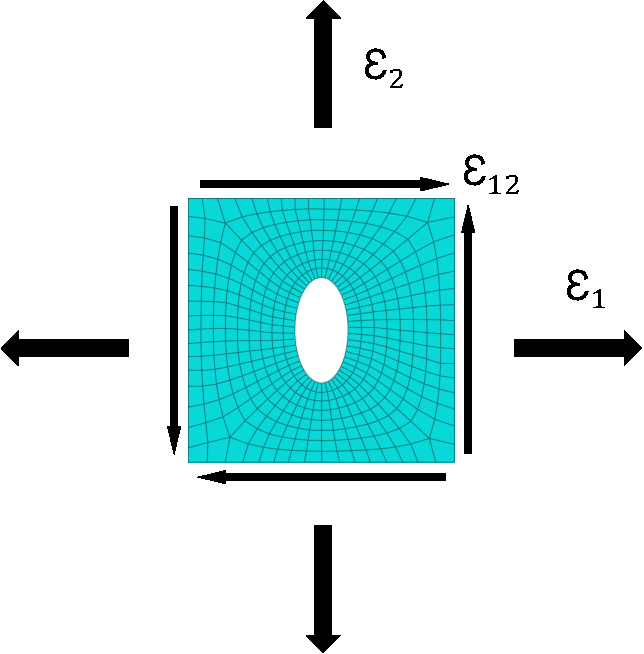
\includegraphics[width=.3\textwidth]{pics/ohcp-geom-loads.pdf}
\end{figure}

% =============================================================================
\section{Results}
% =============================================================================

Before aligning the kernel parameters, SVM with quantum kernels scores similarly to the classical RBF kernel with $\gamma=1$. Furthermore, for low constraint penalty, quantum kernels are close to random guessing.

However, kernel-target alignment improves the mean test accuracy of all quantum kernels both for low and for high constraint strenght, suggesting learning of the OHCP ultimate strength envelope. For higher number of quantum bits (qek0608), quantum kernels show better generalization than classical RBF with optimized $\gamma$.

\begin{figure}[H]
    \centering
    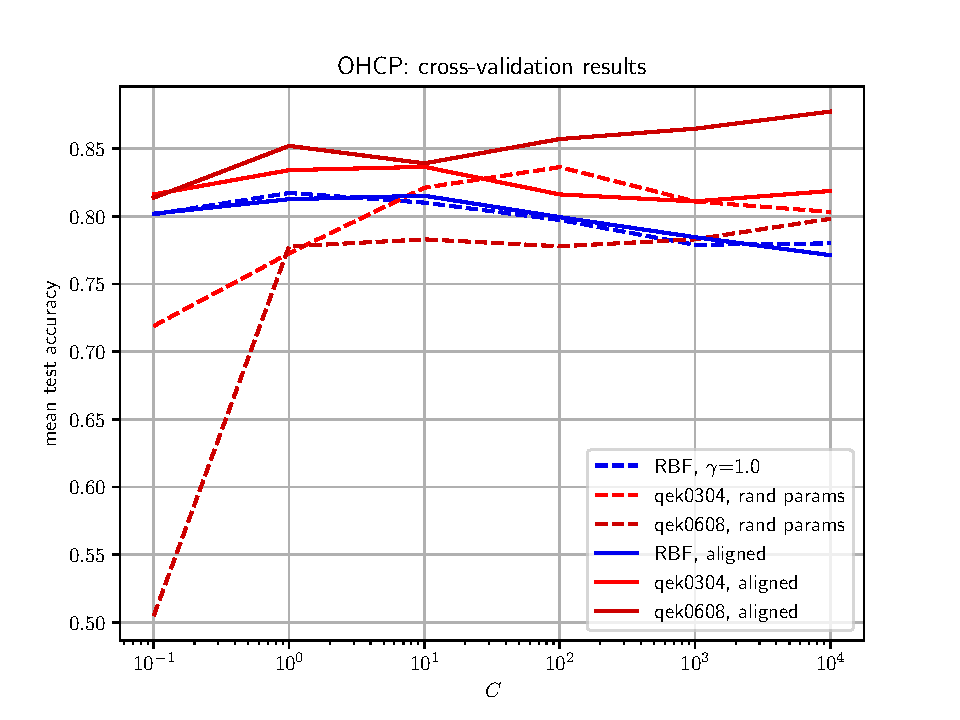
\includegraphics[width=.45\textwidth]{pics/cv-accuracy.pdf}
\end{figure}
% =============================================================================
% \section{Open questions}
% =============================================================================

% =============================================================================
% references
% =============================================================================

\begin{thebibliography}{99}
\bibitem{TGullikers}
    T. Gullikers, \emph{An Integrated Machine Learning and Finite
    Element Analysis Framework, applied to
    Composite Substructures including Damage}, 2018, MSc thesis, TU Delft, Aerospace Structures and Materials.
\bibitem{Havlicek}
    V. Havli\u{c}ek \emph{et al.}, \emph{Supervised Learning with Quantum-Enhanced Feature Spaces}, 2019, Nature.
\end{thebibliography}

% %%%%%%%%%%%%%%%%%%%%%%%%%%%%%%%%%%%%%%%%%%%%%%%%%%%%%%%%%%%%%%%%%%%%%%%%%%%%%
\end{multicols}
\end{document}
% %%%%%%%%%%%%%%%%%%%%%%%%%%%%%%%%%%%%%%%%%%%%%%%%%%%%%%%%%%%%%%%%%%%%%%%%%%%%%